\documentclass{article}
\usepackage{amsmath, sfmath, multicol, tkz-euclide, array, enumerate, tcolorbox, tabularray, tipa}
\renewcommand{\familydefault}{\sfdefault}
\setlength{\parindent}{0cm}
\pagestyle{empty}
\usepackage[left=1in, top=0.5in, right=1in, bottom=0.5in]{geometry}
\tikzset{>=stealth, label style/.append style={font=\footnotesize}}
\tcbset{colback=white}

\newcounter{example}[section]
\newenvironment{example}[1][]{\refstepcounter{example}\par\medskip
   {\color{red}\textbf{Example~\theexample. #1}}}{\medskip}

\newcommand{\arc}[1]{%
    \setbox9=\hbox{#1}%
    \ooalign{\resizebox{\wd9}{\height}{\texttoptiebar{\phantom{A}}}\cr#1}}

\begin{document}

\section*{Areas of Quadrilaterals}

\begin{tcolorbox}[colframe=orange!70!white, coltitle=black, title=\textbf{Today I Can}]
\begin{enumerate}
    \item Find the area of quadrilaterals.
\end{enumerate}
\end{tcolorbox}
\smallskip 

\begin{tabular}{p{0.3\textwidth}p{0.3\textwidth}p{0.3\textwidth}}
\textbf{Parallelogram}   &   \textbf{Rectangle}   &   \textbf{Square}  \\[8pt]
% Parallelogram
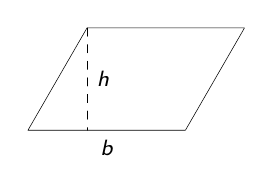
\begin{tikzpicture} 
\tkzDefPoints{0/0/A, 2/0/B}
\tkzDefShiftPoint[A](60:1.5){D}
\tkzDefShiftPoint[B](60:1.5){C}
\tkzDrawPolygon(A,B,C,D)
\tkzLabelSegment[below](A,B){$b$}
\tkzDefLine[orthogonal = through D](D,C)
\tkzGetPoint{E}
\tkzInterLL(D,E)(A,B)
\tkzGetPoint{F}
\tkzDrawSegment[dashed](D,F)
\tkzLabelSegment[right](D,F){$h$}
\end{tikzpicture}
&
% Rectangle
\begin{tikzpicture}
\tkzDefPoints{0/0/A, 2/0/B, 2/1/C, 0/1/D}
\tkzMarkRightAngle(C,B,A)
\tkzDrawPolygon(A,B,C,D)
\tkzLabelSegment[below](A,B){$b$}
\tkzLabelSegment[right](B,C){$h$}
\end{tikzpicture}
&
% Square
\begin{tikzpicture}[scale=0.9]
\tkzDefPoints{0/0/A, 2/0/B, 2/2/C, 0/2/D}
\tkzMarkRightAngle(C,B,A)
\tkzDrawPolygon(A,B,C,D)
\tkzLabelSegment[right](B,C){$s$}
\end{tikzpicture}
\\[0.2in]
$A=bh$  &   $A=bh$  &   $A=s^2$ \\[0.25in]
\textbf{Rhombus} &   \textbf{Kite}    &   \textbf{Trapezoid}    \\
% Rhombus
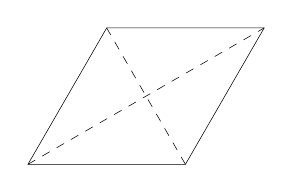
\begin{tikzpicture}
\tkzDefPoints{0/0/A, 2/0/B}
\tkzDefShiftPoint[A](60:2){D}
\tkzDefShiftPoint[B](60:2){C}
\tkzDrawPolygon(A,B,C,D)
\tkzDrawSegments[dashed](A,C B,D)
\end{tikzpicture}
&
% Kite
\begin{tikzpicture}[scale=0.9]
\tkzDefPoints{0/0/A, 3.5/0/C, 1.25/1.25/B, 1.25/-1.25/D}
\tkzDrawPolygon(A,B,C,D)
\tkzDrawSegments[dashed](A,C B,D)
\end{tikzpicture}
&
% Trapezoid
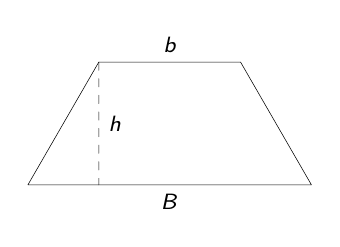
\begin{tikzpicture}[scale=0.9]
\tkzDefPoints{0/0/A, 4/0/B}
\tkzDefShiftPoint[A](60:2){D}
\tkzDefShiftPoint[B](120:2){C}
\tkzDrawPolygon(A,B,C,D)
\tkzLabelSegment[above](C,D){$b$}
\tkzLabelSegment[below](A,B){$B$}
\tkzDefLine[orthogonal = through D](C,D)
\tkzGetPoint{E}
\tkzInterLL(D,E)(A,B)   \tkzGetPoint{F}
\tkzDrawSegment[dashed](D,F)
\tkzLabelSegment[right](D,F){$h$}
\end{tikzpicture}
\\[0.25in]
$A=\frac{1}{2}d_1d_2$   &   $A=\frac{1}{2}d_1d_2$   &
$A=\frac{1}{2}h(b+B)$
\end{tabular}

\bigskip 

\begin{example}
Find the area of each quadrilateral.  \newline\\

\begin{tabular}{p{0.3\textwidth}p{0.3\textwidth}p{0.3\textwidth}}
(a) &   (b) &   (c) \\
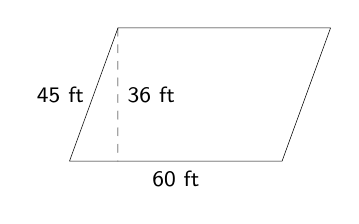
\begin{tikzpicture}[scale=0.9]
\tkzDefPoints{0/0/A, 3/0/B}
\tkzDefShiftPoint[A](70:2){D}
\tkzDefShiftPoint[B](70:2){C}
\tkzDrawPolygon(A,B,C,D)
\tkzDefLine[orthogonal = through D](D,C)
\tkzGetPoint{E}
\tkzInterLL(D,E)(A,B)
\tkzGetPoint{F}
\tkzDrawSegment[dashed](D,F)
\tkzLabelSegment[below](A,B){60 ft}
\tkzLabelSegment[left](A,D){45 ft}
\tkzLabelSegment[right](D,F){36 ft}
\end{tikzpicture}
&
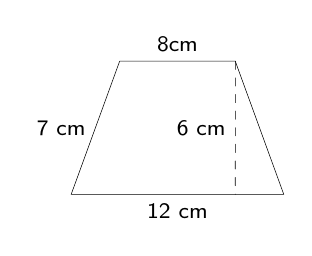
\begin{tikzpicture}[scale=0.9]
\tkzDefPoints{0/0/A, 3/0/B}
\tkzDefShiftPoint[A](70:2){D}
\tkzDefShiftPoint[B](110:2){C}
\tkzDrawPolygon(A,B,C,D)
\tkzDefLine[orthogonal = through C](C,D)
\tkzGetPoint{E}
\tkzInterLL(C,E)(A,B)   \tkzGetPoint{F}
\tkzDrawSegment[dashed](C,F)
\tkzLabelSegment[left](C,F){6 cm}
\tkzLabelSegment[below](A,B){12 cm}
\tkzLabelSegment[above](C,D){8cm}
\tkzLabelSegment[left](A,D){7 cm}
\end{tikzpicture}
&
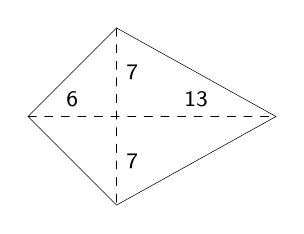
\begin{tikzpicture}[scale=0.9]
\tkzDefPoints{0/0/A, 3.5/0/C, 1.25/1.25/B, 1.25/-1.25/D}
\tkzDrawPolygon(A,B,C,D)
\tkzDrawSegments[dashed](A,C B,D)
\tkzInterLL(A,C)(B,D)   \tkzGetPoint{E}
\tkzLabelSegments[right](B,E D,E){7}
\tkzLabelSegment[above](A,E){6}
\tkzLabelSegment[above](E,C){13}
\end{tikzpicture}
\end{tabular}
\end{example}

\vfill 

Occasionally, we will have to make use of trigonometry in order to find the area.

\vspace{0.5in}
\newpage 

\begin{example}
Find the area of each quadrilateral. Round your answers to 2 decimal places. \newline\\

\begin{tabular}{p{0.3\textwidth}p{0.3\textwidth}p{0.3\textwidth}}
(a) &   (b) &   (c) \\
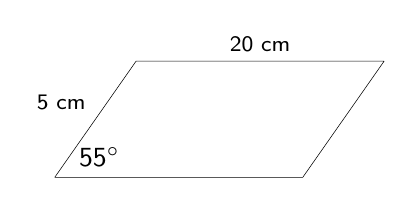
\begin{tikzpicture}[scale=0.9]
\tkzDefPoints{0/0/A, 3.5/0/B}
\tkzDefShiftPoint[A](55:2){D}
\tkzDefShiftPoint[B](55:2){C}
\tkzDrawPolygon(A,B,C,D)
\tkzLabelSegment[above](D,C){20 cm}
\tkzLabelSegment[above left](A,D){5 cm}
\tkzLabelAngle[pos=0.65, xshift=0.1cm, yshift=-0.1cm](C,A,D){$55^\circ$}
\end{tikzpicture}
&
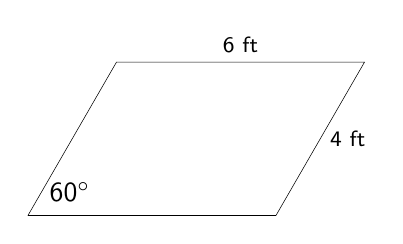
\begin{tikzpicture}[scale=0.9]
\tkzDefPoints{0/0/A, 3.5/0/B}
\tkzDefShiftPoint[A](60:2.5){D}
\tkzDefShiftPoint[B](60:2.5){C}
\tkzDrawPolygon(A,B,C,D)
\tkzLabelSegment[above](D,C){6 ft}
\tkzLabelSegment[right](B,C){4 ft}
\tkzLabelAngle[pos=0.65, xshift=0.1cm, yshift=-0.1cm](C,A,D){$60^\circ$}
\end{tikzpicture}
&
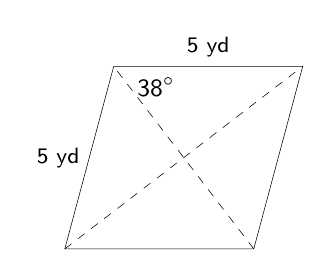
\begin{tikzpicture}[scale=0.8]
\tkzDefPoints{0/0/A, 3/0/B}
\tkzDefShiftPoint[A](75:3){D}
\tkzDefShiftPoint[B](75:3){C}
\tkzDrawPolygon(A,B,C,D)
\tkzDrawSegments[dashed](A,C B,D)
\tkzInterLL(A,C)(B,D)   \tkzGetPoint{E}
\tkzLabelSegment[left](A,D){5 yd}
\tkzLabelSegment[above](C,D){5 yd}
\tkzLabelAngle[pos=0.75](B,D,C){\small $38^\circ$}
\end{tikzpicture}
\end{tabular}
\end{example}

\vfill 

\begin{example}
Find the value of $x$ for each quadrilateral with the given area.
\newline\\

\begin{tabular}{p{0.45\textwidth}p{0.45\textwidth}}
(a) Area = 500 sq. units  &   (b) Area = 40 sq. units  \\[0.2in]
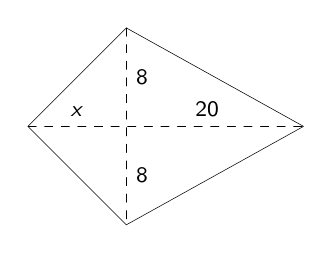
\begin{tikzpicture}
\tkzDefPoints{0/0/A, 3.5/0/C, 1.25/1.25/B, 1.25/-1.25/D}
\tkzDrawPolygon(A,B,C,D)
\tkzDrawSegments[dashed](A,C B,D)
\tkzInterLL(A,C)(B,D)   \tkzGetPoint{E}
\tkzLabelSegments[right](B,E D,E){8}
\tkzLabelSegment[above, xshift=-0.1cm](C,E){20}
\tkzLabelSegment[above](A,E){$x$}
\end{tikzpicture}
&
\begin{tikzpicture}
\tkzDefPoints{0/0/A, 4/0/B}
\tkzDefShiftPoint[A](60:2){D}
\tkzDefShiftPoint[B](120:2){C}
\tkzDrawPolygon(A,B,C,D)
\tkzLabelSegment[above](C,D){$x$}
\tkzLabelSegment[below](A,B){11}
\tkzDefLine[orthogonal = through D](C,D)
\tkzGetPoint{E}
\tkzInterLL(D,E)(A,B)   \tkzGetPoint{F}
\tkzDrawSegment[dashed](D,F)
\tkzLabelSegment[right](D,F){5}
\end{tikzpicture}
\end{tabular}
\end{example}

\vfill 
\end{document}
